\part{Theorie}
\chapter{Kansrekenen}
De kans op een gebeurtenis A:
$$P(A) = \frac{\hbox{\# gunstige gevallen}}{\hbox{tot \# mogelijkheden}}$$
Altijd geldig: 
$$0 \leq P(A) \leq 1$$
\section{Bewerkingen}
\begin{enumerate}
	\item $P(A \cap B)$: kans op gebeurtenis A en gebeurtenis B
	\item $P(A \cup B)$: kans op gebeurtenis A of gebeurtenis B
	\item $P(A|B)$: Voorwaardelijke kans (lees: Wat is de kans op A indien B waar is). A en B zijn onafhankelijk indien $P(A|B) = P(A)$ of $P(B|A) = P(B)$
\end{enumerate}
\section{Rekenregels}
\begin{enumerate}
	\item Optellingswet: $P(A \cup B) = P(A) + P(B) - P(A \cap B)$
	\item Vermenigvuldigingswet: $P(A \cap B) = P(A)P(B)$
	\item Complementswet: $P(\overline{A}) = 1 - P(A)$
	\item $P(A \cap \overline{B}) = P(A) - P(A \cap B)$
\end{enumerate}
\example{Wat is $P(A\cup B\cup C)$?}
{
	\begin{equation*}
		\begin{split}
			& P(A\cup B\cup C)\\
			= & P(A\cup B) + P(C) - P[(A \cup B) \cap C]\\
			= & P(A) + P(B) - P(A\cap B) + P(C) - P[(A \cap B) \cup (B \cap C)]\\
			= & P(A) + P(B) + P(C) - P(A \cap B) - [P(A \cap C) + P(B \cap C) - P(A \cap B \cap C)]\\
			= & P(A) + P(B) + P(C) - P(A \cap B) - P(A \cap C) - P(B \cap C) + P(A \cap B \cap C)
		\end{split}
	\end{equation*}
}



\section{Combinatieleer}
De permutatie(volgorde is van belang): $$P_n = n!$$ (Op hoeveel verschillende manieren kunnen we 5 studenten plaatsen op 5 stoelen \textbf{OF} het aantal verschillende manieren om \textit{n} elementen te ordenen)


De combinatie(volgorde is niet van belang): $$C_n^p = (_p^n) = \frac{n!}{p!(n - p)!}$$ (Op hoeveel verschillende manieren kunnen we 2 studenten kiezen uit 5 \textbf{OF} het aantal verschillende manieren om \textit{p} elementen te kiezen uit \textit{n}.)

\example{In een vaas zitten 8 rode, 4 witte en 3 blauwe knikkers. Wat is de kans om met trekken met teruglegging exact 2 rode knikkers te nemene bij het trekken van 5 knikkers?}{
	$$P(2R) = \frac{8}{15} \cdot \frac{8}{15} \cdot \frac{7}{15} \cdot \frac{7}{15} \cdot \frac{7}{15} \cdot C_5^2$$
	
	Het getal $\frac{8}{15}$ stelt de kans voor om een rode knikker te trekken. Het getal $\frac{7}{15}$ stelt de kans voor om geen rode knikker te trekken. Er wordt vermenigvuldigt met $C_5^2$ de 2 rode knikkers elk van de 5 plaatsen kunnen innemen.
	$$=C_5^2 \bigg(\frac{8}{15}\bigg)^2\bigg(\frac{7}{15}\bigg)^3$$
	$$= 10 \cdot \frac{64}{225} \cdot \frac{343}{3375} = 0.29 = 29\%\; \hbox{kans}$$
	
}

\section{Regel van Bayes}
$$P(A_j|B) = \frac{P(A_j \cap B)}{P(B)} = \frac{P(A_j)P(B|A_j)}{\sum_{i = 1}^{n}P(A_i)P(B|A_i)}$$

\example{In een jaszak zitten 2 munten: één normaal(N) en één vervalst(V) (munt aan elke zijde). Een muntstuk wordt aselect gekozen en gegooid. Munt komt bovenaan te liggen. Wat is de kans dat dit het normale muntstuk is? Dit muntstuk wordt opnieuw gegooid. Terug munt. Wat is nu de kans dat dit het normale muntstuk is?}{
	
	$$P(N) = \frac{1}{2}$$
	$$P(V) = \frac{1}{2}$$
	\\
	De kans dat het munt of kop is bij het normale muntstuk is 0.5.
	$$P(M/N) = P(K/N) = \frac{1}{2}$$
	De kans dat het munt is bij het valse muntstuk is 1.
	$$P(M/V) = 1$$
	Regel van Bayes:
	\begin{equation*}
	 \begin{split}
	  P(N/M) & = \frac{P(N)P(M/N)}{P(M/N)P(N) + P(M/V)P(V)}\\
	         & = \frac{\frac{1}{2} \cdot \frac{1}{2}}{\frac{1}{2} \cdot \frac{1}{2} + 1\cdot \frac{1}{2}}
	          = \frac{\frac{1}{4}}{\frac{3}{4}}
	          = \frac{1}{3}
	 \end{split}
	\end{equation*}
	Indien muntstuk opnieuw wordt gegooid:
	\begin{equation*}
	 \begin{split}
	   P(N/2M) & = \frac{P(N)P(2M/N)}{P(2M/N)P(N) + P(2M/V)P(V)}\\
	           & = \frac{\frac{1}{2} \cdot (\frac{1}{2} \cdot \frac{1}{2})}{(\frac{1}{2} \cdot \frac{1}{2}) \cdot \frac{1}{2} + 1\cdot \frac{1}{2}}\\
	           & = \frac{\frac{1}{4}}{\frac{5}{4}} = \frac{1}{5}
	 \end{split}
	\end{equation*}
}

\chapter{Beschrijvende statistiek}
\section{Populaties en steekproeven}
\begin{itemize}
	\item \textbf{Populatie}: Een verzameling van elementen 
	\item \textbf{Steekproef}: Een deelverzameling van de populatie. Deze moet representatief zijn (bv $3/4$ van de populatie is vrouw. In de steekproef moet ook $3/4$ vrouw zijn)
\end{itemize}
\section{Veranderlijken}
\begin{itemize}
	\item {\textbf{Stochastische variabele}: Kan waarden aannemen elk met een bepaalde kans.}
	\item {\textbf{Kwalitatieve variabele}: Geen numerieke waarden (bloedgroep, studierichting)}
	\item {\textbf{Kwantiatieve variabele}: Numerieke waarden (gewicht, leeftijd)}
	\item {\textbf{Ordinale variabele}: Er kan een bepaalde orde toegekend worden (zeer goed, goed, matig, voldoende, slecht en zeer slecht)}
	\item {\textbf{Nominale variabele}: Er kan geen bepaalde orde toegekend worden (studierichting)}
	\item {\textbf{Onafhankelijke variabele}: De ene meting beïnvloed de andere niet (gooien van een dobbelsteen)}
	\item {\textbf{Afhankelijke variabele}: De ene meting beïnvloed de andere (grootte per geslacht)}
	\item {\textbf{Discrete variabele}: Heeft enkel discrete waarden (1, 0.4, 7, 9 , 1/100)}
	\item {\textbf{Continue variabele}: Heeft continue waarden ($\sqrt{2}$, $[-10, 10]$)}
\end{itemize}
\section{Discrete veranderlijken}
\subsection{Ordenen van gegevens}
Stel \textit{n} het aantal elementen van de populatie of van een steekproef en \textit{k} het aantal verschillende waarden dat de veranderlijke kan aannemen.
$$\sum_{i=1}^{k} n_i = n$$
\begin{itemize}
	\item {\textbf{Absolute frequentie}: Het aantal keer dat een bepaalde waarde aangenomen wordt.
			
	}
	\item {\textbf{Relatieve frequentie}: De verhouding van de absolute frequentie tot het aantal elementen
		$$f_i = \frac{n_i}{n}\;\;\;\hbox{en}\;\;\;\sum_{i = 1}^{k} f_i = 1$$
	}
	\item {\textbf{Cumulatieve absolute frequentie}: 
		$$N_i = \sum_{j=1}^{i} n_j$$
	}
	\item {\textbf{Cumulatieve relatieve frequentie}:
		$$F_i = \sum_{j=1}^{i} f_i$$
	}
	\item {\textbf{Frequentietabel}: Voorstelling van alle frequenties.\\
		Een toets bij 204 studenten, gequoteerd op 10, leverde volgende resultaten:\\
		\begin{tabular}{l | l l l l l l l l l}
			score & 2 & 3 & 4  & 5  & 6  & 7  & 8  & 9  & 10 \\
			\hline
			$n_i$ & 1 & 5 & 16 & 21 & 39 & 44 & 50 & 26 & 2  
		\end{tabular}\\
		De frequentietabel wordt:\\
		\begin{tabular}{l | l | l | l | l | l | l | l | l | l}
			score & 2     & 3     & 4     & 5     & 6     & 7     & 8     & 9     & 10   \\
			\hline
			$n_i$ & 1     & 5     & 16    & 21    & 39    & 44    & 50    & 26    & 2    \\
			$f_i$ & 0.005 & 0.025 & 0.078 & 0.103 & 0.191 & 0.216 & 0.245 & 0.127 & 0.01 \\
			$N_i$ & 1     & 6     & 22    & 43    & 82    & 126   & 176   & 202   & 204  \\
			$F_i$ & 0.005 & 0.029 & 0.108 & 0.211 & 0.402 & 0.618 & 0.863 & 0.990 & 1    
		\end{tabular}
	}
\end{itemize}
\subsection{Plaatsparameters en spreidingsparameters}
\begin{itemize}
	\item {\textbf{Steekproefgemiddelde}: De som van alle waarnemingen gedeeld door het totaal aantal waarnemingen
		$$\overline{x} = \frac{1}{n}(x_1 + x_2 + ... + x_n) = \frac{1}{n} \sum_{i = 1}^{n} = x_i$$
	}
	\item {\textbf{Modus}: De waarde met de grootste absolute frequentie.}
	\item {\textbf{Mediaan}: Na orderning van de waarnemingen, de middelste waarde als n oneven is en het gemiddelde van de middelste twee als n even is.}
	\item {\textbf{Variantie}: Het rekenkundig gemiddelde van de \textbf{kwadraten van de afwijkingen} van de waarnemingsgetallen ten op zichte van hun rekenkundig gemiddelde:
		$$s^2 = \frac{1}{n - 1}\sum_{i=1}^{n}(x_i - \overline{x})^2$$}
	\item {\textbf{Standaardafwijking}: De vierkantswortel uit de steekproefvariantie. 
		$$\sigma = \sqrt{s^2} = s$$}
\end{itemize}
\section{Continue veranderlijken}
\subsection{Ordenen van gegevens}
Het ordenen van continue veranderlijken wordt gedaan met klassen.
\begin{itemize}
	\item {\textbf{Spreidingsbreedte (range)}: Het verschil tussen het grootste en het kleinste waarnemingsgetal.}
	\item {\textbf{Aantal klassen}: Het aantal klassen is de vierkantswortel uit het aantal elementen: $$k = \sqrt{n}$$}
	\item {\textbf{Klassebreedte ($\Delta x$)}: De breedte van elke klasse. Indien elke klasse een verschillende breedte heeft wordt $\Delta x_i$ gebruikt om de \textit{i}-de klasse aan te duiden.}
	\item {De frequenties zijn analoog aan discrete veranderlijken}
\end{itemize}

\subsection{Plaatsparameters en spreidingsparameters}
\begin{itemize}
	\item {\textbf{Het rekenkundig gemiddelde}: 
		$$\overline{x} = \frac{1}{n}\sum_{i=1}^{k}n_ic_i$$
		met $c_i$ het klassemidden van de \textit{i}-de klasse.
	}
	\item {\textbf{De modale klasse}: De klasse met de grootste absolute frequentie.}
	\item {\textbf{De mediale klasse}: De klasse met de laagste waarden waarin de cumulatieve relatieve frequentie minstens 0.5 bedraagt}
	\item {\textbf{De variantie}:
		$$s^2 = \frac{1}{n-1}\sum_{i=1}^{k}n_i(c_i-\overline{x})^2$$
	}
	\item {\textbf{Standaardafwijking}:
		$$\sigma = \sqrt{s^2} = s$$}
\end{itemize}

\subsection{Momenten van een steekproef}
\todo{epic}

\chapter{Verdelingsfuncties van een populatie}
Twee soorten verdelingsfuncties:
\begin{itemize}
	\item Kansfunctie: bij discrete kansen (sommeren)
	\item Dichtheidsfunctie: bij continue kansen (integreren)
\end{itemize}
\section{Kansfunctie}
De kansfunctie $f(x)$:
$$f(x_i) = P(X = x_i) \qquad \hbox{met}\qquad i = 1, 2, ..., k$$
$$f(x) = 0 \qquad \hbox{als} \qquad k \notin \{x_1, ..., x_n\}$$
De som van alle kansen is gelijk aan 1:
$$\sum_{i = 1}^{k} f(x_i) = 1$$
De cumulatieve distributiefunctie wordt gegeven door:
$$F(x) = P(x \leq t) = \sum_{x_i \leq t} f(x_i)\;dx$$
\section{Dichtheidsfunctie}
De som van alle kansen is gelijk aan 1:
$$\int_{-\infty}^{+\infty} f(x)\;dx = 1$$
Aangezien we integreren:
$$\int_{a}^{a} f(x)\;dx = 0$$
Hieruit volgt:
\begin{equation*}
	\begin{split}
		& P(a \leq x \leq b) \\
		= & P(a < x \leq b)  \\
		= & P(a < x < b)     \\
		= & P(a \leq x < b)
	\end{split}
\end{equation*}
De cumulatieve distributiefunctie wordt gegeven door:
$$F(x) = P(x \leq t) = \int_{-\infty}^{t} f(x)\;dx$$
\example{Stel $f(x) = 
	\begin{cases} 
		a + b(x - 1)^2  & 0 \leq x \leq 2
		               \\ 0 &  anders 
		
	\end{cases}$.\\ 
	Bepaal a en b zodat f een geldige dichtheidsfunctie is. Bepaal ook $F(t)$.}{
	
	\begin{equation*}
		\begin{split}
			\int_{-\infty}^{+\infty} f(x)\; dx = 1 
			& \Leftrightarrow \int_{0}^{2} a + b(x - 1)^3 \; dx = 1 \\
			& \Leftrightarrow ax + b\frac{(x - 1)^4}{4}\bigg|_{0}^{2} = 1 \\
			& \Leftrightarrow 2a + \frac{b}{4}(1 - 1) = 2 \\
			& \Leftrightarrow a = \frac{1}{2}
		\end{split}
	\end{equation*}
	
	Is $f(x) \geq 0\;\forall\;x$?
	\\
	Is $\frac{1}{2} + b(x - 1)^3 \geq 0$? $(x \in [0, 2])$
	$$\Rightarrow x \in [0, 2] \Rightarrow -1 \leq (x - 1)^3 \leq 1$$
	
	\underline{Als $b > 0$:}
	$$- b \leq b(x-1)^3 \leq b$$
	$$\frac{1}{2} - b \leq b(x-1)^3 + \frac{1}{2} \leq b + \frac{1}{2}$$
	$f(x)$ zal $\geq 0$ indien $\frac{1}{2} - b \geq 0$
	$$\Rightarrow b \leq \frac{1}{2}$$
	
	\underline{Als $b < 0$:}
	\begin{equation*}
		\begin{split}
			- b \geq b(x-1)^3 \geq b & \Rightarrow b \leq b(x-1)^3 \leq -b \\
			& \Rightarrow b + \frac{1}{2} \leq b(x-1)^3+ \frac{1}{2}  \leq -b + \frac{1}{2}
		\end{split}
	\end{equation*}
	$f(x)$ zal $\geq 0$ indien $\frac{1}{2} + b \geq 0$
	$$\Rightarrow b \geq -\frac{1}{2}$$
	
	\begin{equation*}
	 \begin{split}
	  F(t) & = \int_{0}^{t} \frac{1}{2} + b(x - 1)^3\; dx \;\; (t \in [0, 2])\\
	       & = \frac{1}{2}x + b\frac{(x-1)^4}{4}\bigg|_{0}^{t} \\
	       & = \frac{1}{2}t + \frac{b}{4}[(t-1)^4 - 1]
	 \end{split}
	\end{equation*}
	Bovendien is $F(t) = 0$ als $t < 0$ en is $F(t) = 1$ als $t > 2$
	
}

\section{Plaatsparameters}
Van een variabele x kennen we de dichtheidsfunctie $f(t)dt$ die de kans epaalt dat x een waarde in het interval $[t, t + dt]$ aanneemt. Voor een willekeurige functie $g(x)$ defineert men de verwachte waarde als volgt:
\begin{itemize}
 \item Discreet: $$E[g(x)] = \sum_{i = 1}^{k} g(x_{i})f(x_i)$$
 \item Continu: $$\int_{-\infty}^{+\infty}g(x)f(x)\; dx$$
\end{itemize}


\example{Wat is de gemiddelde waarde bij het gooien van een dobbelsteen}{
  \begin{equation*}
   \begin{split}
    \mu & = 1\cdot\frac{1}{6} + 2\cdot\frac{1}{6} +3\cdot\frac{1}{6} +4\cdot\frac{1}{6} +5\cdot\frac{1}{6}+ 5\cdot\frac{1}{6}\\
    &= 3.5
   \end{split}
  \end{equation*}
}
\example{Bepaal de gemiddelde winst als bij kop 3 euro wordt betaald en bij munt 5 euro. Het munstuk is vervalst zodat P(k) = 2P(M)}{
We maken een stelsel op met 2 formules. De extra formule is de som van alle kansen die gelijk is aan 1.
$$\begin{cases}
   P(K) = 2P(M) \\
   P(K) + P(M) = 1
  \end{cases}
$$
Hieruit wordt afgeleid dat 
\begin{equation*}
 \begin{split}
   P(K) &= \frac{2}{3} \\
   P(M) &= \frac{1}{3}
 \end{split}
\end{equation*}
De winstfunctie wordt gedefinieerd als g met g(K) = 3 en g(M) = 5.
\begin{equation*}
 \begin{split}
  E[g(x)] & = g(K)\cdot P(K) + g(M)\cdot P(M)\\
          & = 3 \cdot \frac{2}{3} + 5 \cdot \frac{1}{3}\\
          & = 2 + \frac{5}{3}\\
          & = \frac{11}{3}
 \end{split}
\end{equation*}
}
\example{Bereken de gemiddelde winst x met F(x) zoals grafisch weergegeven 
\begin{center}
 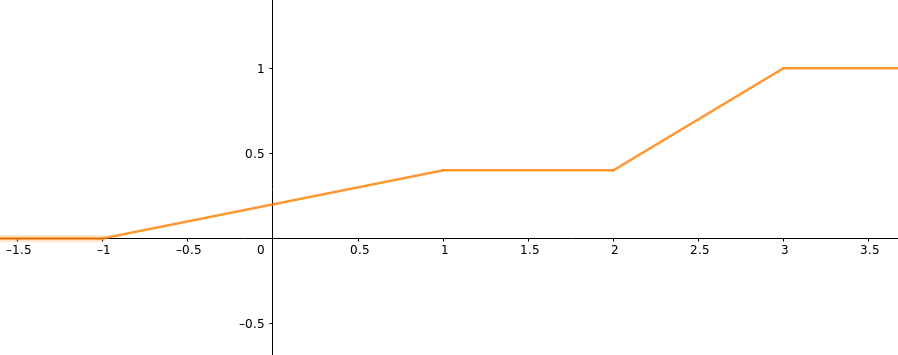
\includegraphics[width=0.5\linewidth]{slide_7}
\end{center}

}{
\begin{equation*}
 \begin{split}
  \mu & = E[x] \\
      & = \int_{-1}^{1} x\cdot f(x)\; dx + \int_{2}^{3} x\cdot f(x)\; dx
 \end{split}
\end{equation*}
De functie kan gedefinieerd worden als:
$$F(x) = \begin{cases}
   0.2(x + 1) & x \in [-1,1] \\
   1 + 0.6(x-3) & x \in [2,3] \\
   0 & x < -1 \\
   1 & x > 3 \\
   0.4 & x \in [1, 2]
\end{cases}$$
We weten dat $f(x) = \frac{dF(x)}{dx}$. We leiden $F(x)$ af voor de intervallen $[-1, 1]$ en $[2, 3]$ 
\begin{equation*}
      \begin{split}
       \mu & = \int_{-1}^{1} x\cdot \frac{1}{5}\; dx + \int_{2}^{3} x\cdot \frac{3}{5}\; dx \\
           & = \frac{x^2}{10}\bigg|_{-1}^{1} + \frac{3x^2}{10}\bigg|_{2}^{3} \\
           & = \frac{1}{10}\bigg[(1 - 1) + 3(9 - 4)      \bigg] \\
           & = \frac{15}{10} = \frac{3}{2}
      \end{split}
\end{equation*}
}
\example{Bereken de mediaan van x
\begin{center}
 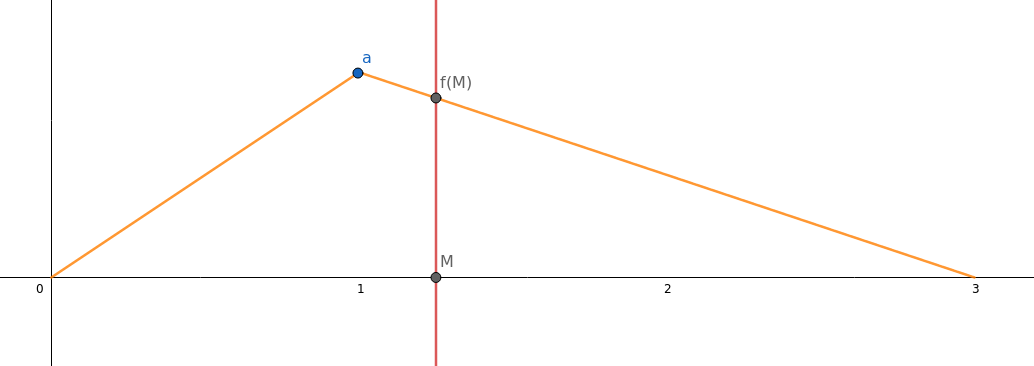
\includegraphics[width=0.90\textwidth]{oef_mediaan}
\end{center}
}{
De oppervlakte van het rechterdeel moet gelijk zijn aan 50\%. We gebruiken de formule van de oppervlakte van een driehoek.

\begin{equation*}
 \begin{split}
  &  \frac{(3 - M) \cdot f(M)}{2} = \frac{1}{2} \\
  \Leftrightarrow & (3 - M) \cdot f(M) = 1
 \end{split}
\end{equation*}
De som van alle kansen moet gelijk zijn aan 1.
\begin{equation*}
 \begin{split}
  \int_{0}^{3}f(x)\;dx = 1 & \Leftrightarrow \frac{a}{2} + a = 1\\
  & \Leftrightarrow a = \frac{2}{3}
 \end{split}
\end{equation*}
De rechte door $(2, \frac{2}{3})$ en $(3, 0)$ wordt gegeven door 
$$y = -\frac{1}{3}(x-3)$$
Herschrijf:
$$f(M) = -\frac{1}{3}(M - 3)$$
Nu kan de formule van de oppervlakte van de driehoek terug gebruikt worden:
\begin{equation*}
 \begin{split}
  & (3 - M)(-\frac{1}{3}(M - 3)) = 1  \\
  \Leftrightarrow & M = 3 \pm \sqrt{3}\\
  \Leftrightarrow & M = 3 - \sqrt{3} \;\;\;\hbox{(aangezien de functie niet hoger gaat dan 3)}
  \end{split}
\end{equation*}
}

\section{Spreidingsparameters}
De variantie:
\begin{itemize}
 \item \textbf{Continu}: $$\sigma^2 = V[x] = \int_{-\infty}^{+\infty}(x-\mu)^2 f(x)\; dx$$
 \item \textbf{Discreet}: $$\sigma^2 = V[x] = \sum_{i}(x_i - \mu)^2 f(x_i)$$
\end{itemize}
De standaardafwijking blijft $\sigma = \sqrt{\sigma^2}$

\example{Bewijs $V[ax + b] = a^2V[x]$}{
We bewijzen enkel voor een continue dichtheidsfunctie, maar is analoog aan discrete kansfuncties.

\begin{equation*}
 \begin{split}
  V[ax + b] & = \int_{-\infty}^{+\infty}(ax + b - a\mu + b)^2 f(x)\; dx \\
            & = \int_{-\infty}^{+\infty}a^2(x - \mu)^2 f(x)\; dx \\
            & = a^2\int_{-\infty}^{+\infty}(x - \mu)^2 f(x)\; dx \\
            & = a^2V[x]
 \end{split}
\end{equation*}
}
\example{Bewijs $V[x] = E[x^2] - \mu^2$}{
\begin{equation*}
 \begin{split}
  V[x] & = E[(x - \mu)^2] \\
       & = E[x^2 - 2x\mu + \mu^2] \\
       & = E[x^2] - E[2x\mu] + E[\mu^2] \\
       & = E[x^2] - 2\mu E[x] + \mu^2E[1] \\
       & = E[x^2] - 2\mu^2 + \mu^2 \\
       & = E[x^2] - \mu^2
 \end{split}
\end{equation*}


}

\section{Momenten}
Het moment van de orde k ten opzichte van het punt c:
$$E[(x - c)^k]$$
Er bestaan 2 gevallen voor c.
\begin{itemize}
 \item $c = 0\;:\; \mu'_{k} = E[x^k]$
 \item $c = \mu \;:\; \mu_k = E[(x - \mu)^k]$
\end{itemize}
Een aantal voorbeelden:
\begin{enumerate}
 \item $\mu'_0 = E[x^0] = E[1] = 1$
 \item $\mu'_1 = E[x^1] = \mu$
 \item $\mu_0 = E[(x - \mu)^0] = E[1] = 1$
 \item $\mu_1 = E[(x - \mu)^1] = E[x] - \mu = 0$
 \item $\mu_2 = E[(x - \mu)^2] = V[x] = \sigma$
\end{enumerate}

\subsection{De momentenfunctie}
De momentenfunctie wordt gedefinieerd als:
$$M(t) = E[e^{tx}]$$
\begin{itemize}
 \item \textbf{Discreet}: $$M(t) = \sum_{i} e^{tx_i} f(x_i)$$
 \item \textbf{Continu}: $$M(t) = \int_{-\infty}^{+\infty} e^{tx} f(x)\; dx$$
\end{itemize}
Wat ook altijd geldig is:
$$E[x^k] = \frac{d^kM(t)}{dt^k}\bigg|_{t=0}$$
Bewijs:
\begin{equation*}
 \begin{split}
  \frac{dM(t)}{dt}             & = \frac{d}{dt}\int_{-\infty}^{+\infty} e^{tx} f(x)\; dx \bigg|_{t=0} \\
                               & = \int_{-\infty}^{+\infty} xe^{tx} f(x)\; dx \bigg|_{t=0} \\
                               & = \int_{-\infty}^{+\infty} x f(x)\; dx \\
                               & = E[x] \\
                               & = \mu
 \end{split}
\end{equation*}
\begin{equation*}
 \begin{split}
  \frac{d^2M(t)}{dt^2}         & = \frac{d}{dt}\int_{-\infty}^{+\infty} xe^{tx} f(x)\; dx \bigg|_{t=0} \\
                               & = \int_{-\infty}^{+\infty} x^2e^{tx} f(x)\; dx \bigg|_{t=0} \\
                               & = \int_{-\infty}^{+\infty} x^2 f(x)\; dx \\
                               & = E[x^2]
 \end{split}
\end{equation*}
\begin{equation*}
 \begin{split}
  \frac{d^kM(t)}{dt^k}             & = \frac{d}{dt}\int_{-\infty}^{+\infty} x^k f(x)\; dx \\
                                   & = E[x^k]
 \end{split}
\end{equation*}

\example{
        Bereken het gemiddelde en variantie van de geometrische verdeling
    }{
        $i: \#$ herhalingen van een experiment tot dat een gebeurtenis A voor de eerste keer optreedt en $p$ de kans op succes.
        $$f(i) = (1 - p)^{i - 1}p$$
        Controle dat dit een geldige kansfunctie is:
        \begin{equation*}
         \begin{split}
                        \sum_{i = 1}^{+\infty} f(i) = 1 \\
          \Rightarrow & \sum_{i = 1}^{+\infty} (1 - p)^{i - 1}p = 1 \\
          \Rightarrow & p\sum_{i = 1}^{+\infty} (1 - p)^{i - 1} = 1 \qquad \hbox{reeks convergeert naar}\; \frac{1}{1 - (1-p)}\\ 
          \Rightarrow & p\frac{1}{1 - (1-p)} = 1 \\
          \Rightarrow & 1 = 1
         \end{split}
        \end{equation*}
        Het gemiddelde:
        \begin{equation*}
         \begin{split}
          \mu & = \sum_{i=1}^{+\infty} f(i) = \sum_{i = 1}^{+\infty} (1 - p)^{i - 1}p \\
          \Rightarrow & \qquad \hbox{moeilijk te sommeren, dus gebruik alternatief} \\
          \mu & = \frac{dM}{dt}|_{t=0} \\
          M(t) & = \sum_{i = 1}^{+\infty}e^{it}f(i) \\
               & = \sum_{i = 1}^{+\infty}e^{it}(1 - p)^{i - 1}p \\
               & = \sum_{i = 1}^{+\infty} \bigg(e^{t}(1 - p)\bigg)^{i - 1}pe^{t} \qquad \hbox{aangezien} \qquad e^{it} = e^{t(i - 1)}e^{t} \\
               & = pe^{t}\sum_{i = 1}^{+\infty} \bigg(e^{t}(1 - p)\bigg)^{i - 1} \\
               & = \frac{pe^{t}}{1 - e^t(1 - p)} \\
          \mu & = \frac{dM}{dt}|_{t=0} \\
              & = \frac{pe^{t}(-e^t(t - p)) - [1 - e^t(1 - p)]pe^t}{[1 - e^t(1 - p)]^2}\bigg|_{t = 0} \\
              & = \frac{pe^{t}}{[1 - e^t(1 - p)]^2}\bigg|_{t = 0} \\
              & = \frac{p}{[1 - 1 - p]^2}\bigg|_{t = 0} \\
              & = \frac{1}{p}
         \end{split}
        \end{equation*}
        De variantie:
        \begin{equation*}
         \begin{split}
          \sigma^2 & = E[x^2] - \mu^2 \\
                   & = \frac{d^2M}{dt^2}|_{t=0} - \bigg(\frac{1}{p}\bigg)^2 \\
                   & = \frac{pe^t(t - e^t(1 - p))^2 - 2pe^t(1 - e^t(1 - p))}{[1 - e^t(1 - p)]^4}\bigg|_{t = 0} - \bigg(\frac{1}{p}\bigg)^2 \\
                   & = \frac{p^3 - 2p^2(-(1-p))}{p^4} - \bigg(\frac{1}{p}\bigg)^2 \\
                   & = \frac{p + 2(1 - p)}{p^2} - \bigg(\frac{1}{p}\bigg)^2 \\
                   & = \frac{2 - p}{p^2} - \bigg(\frac{1}{p}\bigg)^2 \\
                & = \frac{1 - p}{p^2}
         \end{split}
        \end{equation*}

    }
\section{De ongelijkheid van Chebychev}
Twee ongelijkheden:
$$P(|x - \mu| \geq k\sigma) \leq \frac{1}{k^2}$$
$$P(|x - \mu| < k\sigma) \geq 1 - \frac{1}{k^2}$$
Gebruik enkel deze ongelijkheid als er GEEN informatie is over de verdelingsfunctie.
\example{
    Beschouw een $x$ met $\mu = 1$ en $\sigma^2 = \frac{1}{5}$ en  een symmetrische verdeling rond $\mu$.
    Geef een begrenzing voor $P(0 < x < 2)$ en $P(x \geq 1 + \frac{2}{\sqrt{5}})$
}{
    \begin{equation*}
     \begin{split}
      P(0 < x < 2) & = P(P(|x - 1| < 1) \\
                   & = P(P(|x - \mu| < \sqrt{5}\sigma) \\
                   & \geq 1 - \frac{1}{5} \\
                   & \geq \frac{4}{5}
     \end{split}
    \end{equation*}
    \begin{equation*}
     \begin{split}
      P(x \geq 1 + \frac{2}{\sqrt{5}}) & = P(x - \mu \geq \frac{2}{\sqrt{5}}) \\
                                       & = \frac{1}{2}P(|x - \mu| \geq \frac{2}{\sqrt{5}}) \\
                                       & = \frac{1}{8}
     \end{split}
    \end{equation*}
}
\chapter{Discrete verdelingen}
\section{Uniforme discrete verdeling}
Elke kans is gelijk.

Voorschrift:
$$f(i) = \frac{1}{n} \qquad i \in \{1, 2, 3, ..., n\}$$
Gemiddelde:
\begin{equation*}
 \begin{split}
  \mu & = \sum_{i = 1}^{n}i \frac{1}{n} \\
      & =  \frac{1}{n} \sum_{i = 1}^{n}i\\.
      & =  \frac{1}{n}(1 + 2 + 3 + ... + (n - 1) + n)\\
      & =  \frac{1}{n}\bigg(\frac{n(n + 1)}{2}\bigg)\\ 
      & = \frac{n + 1}{2}
 \end{split}
\end{equation*}
Variantie:
\begin{equation*}
 \begin{split}
  \sigma^2 & = E[x^2] - \mu^2 \\
           & = \bigg(\sum_{i = 1}^{n}i^2 \frac{1}{n}\bigg) - \bigg(\frac{n + 1}{2}\bigg)^2 \\
           & = \frac{1}{n}\bigg(\frac{n(n+1)(2n+1)}{6}\bigg) - \bigg(\frac{n + 1}{2}\bigg)^2 \\
           & = \bigg(\frac{(n+1)(2n+1)}{6}\bigg) - \bigg(\frac{n + 1}{2}\bigg)^2 \\
           & = (n + 1)\bigg(\frac{(2n+1)}{6} - \frac{1}{4}\bigg) \\
           & = \frac{(n + 1)}{12}(4n + 2 - 3n - 3) \\
           & = \frac{n^2 - 1}{12}
 \end{split}
\end{equation*}
\section{Bernouilli experiment}
Enkel twee uitkomsten: Succes of geen succes. Success heeft een kans $p$, geen succes heeft een kans $ 1 - p$.

Het gemiddelde:
\begin{equation*}
 \begin{split}
  \mu & = E[x] \\
      & = \sum_{i = 1}^{2}x_if(x_i) \\
      & = 0(1 - p) + 1p \\
      & = p
 \end{split}
\end{equation*}
De variantie:
\begin{equation*}
 \begin{split}
  \sigma^2 & = V[x^2] = E[x^2] - \mu^2 \\
           & = \bigg[\sum_{i = 1}^{2}x_i^2f(x_i)\bigg] - p \\
           & = 0^2(1 - p) + 1^2(p) - p^2 \\
           & = p(1 - p)
 \end{split}
\end{equation*}
\section{Binomiale Verdeling}
Hoeveel successen zijn er indien $n$ experimenten uitgevoerd worden waarbij elk experiment een kans $p$ heeft om te slagen. De experimenten MOETEN onafhankelijk zijn.

Indien x binomiaal verdeeld: $x : bin(n, p)$

Voorschrift:
$$f(i) = P(x = i) = C_n^ip^i(1 - p)^{n - 1}$$

\example{
    Een arts voert op één dag drie operaties uit die elk slagen met kans 0.9. Wat is de kans op twee succesvolle operaties die dag?
}{
    $x : bin(3, 0.9)$
    \begin{equation*}
     \begin{split}
        f(2) & = P(x = 2) \\
             & = C_3^2(0.9)^2(1 - 0.9) \\
             & \approx \frac{1}{4}
     \end{split}
    \end{equation*}

}

Gemiddelde: $np$

Variantie : $np(1 - p)$
\subsection{Momentenfunctie}
\begin{equation*}
 \begin{split}
  M(t) & = E[e^{ti}] \\
       & = \sum_{i=0}^n e^{ti}C_n^ip^i(1 -p)^{n - 1} \\
       & = \sum_{i=0}^n e^{ti}C_n^i\bigg[(pe^t)^i(1 -p)^{n - 1}\bigg] \\ 
       & = ( 1 - p + pe^t)^n
 \end{split}
\end{equation*}

\subsection{Recursieformule}
\begin{equation*}
 \begin{split}
  f(i + 1) & = C_n^{i + 1}p^{i + 1}(1 - p)^{n- (i + 1)} \\
           & = \frac{n!}{(i + 1)!(n - i - 1)!}p^i(1 -p)^{n - 1} \frac{p}{1 - p} \\
           & = \frac{n!}{i!(n - i)!(i + 1)!}p^i(1 -p)^{n - 1} \frac{p}{1 - p} \\
           & = \frac{n!}{i!(n - i)!}p^i(1 -p)^{n - 1} \cdot \frac{n - 1}{i + 1}\frac{p}{1 - p} \\
           & = f(i) \cdot \frac{(n - 1)p}{(i + 1)(1 - p)}
 \end{split}
\end{equation*}


\section{Geometrische verdeling}
Een discrete veranderlijke 
i
waarmee we het 
aantal keer
weergeven dat  we een experiment 
moeten herhalen 
totdat gebeurtenis A zich 
voordoet
, heeft een 
geometrische verdeling.

Voorschrift:
$$f(i) = (1 - p)^{i - 1}p$$
\example{
    We wensen een gepaste persoon te vinden voor een 
    openstaande betrekking
    We testen meerdere kandidaten totdat een kandidaat 
    geschikt bevonden wordt.
    De kans op ‘niet geschikt’ is 10\%.
    Wat is de kans dat na het testen van vier kandidaten pas 
    de gepaste kandidaat gevonden werd?
}{
    $i : \#$ experimenten totdat 1ste succes voorkomt en $p: 0.9$
    $$f(4) = (1 - p)^3p = (0.1)^30.9$$
}

\section{Hypergeometrische verdeling}
N elementen waarvan M de eigenschap A bezitten.
We trekken n elementen .
Wat is de kans dat i van de n elementen eig. A bezitten?

$$f(i) = \frac{C_M^iC_{N - M}^{n - i}}{C_N^n}$$

\example{ 
    De variabele $p = 0.3$ stelt de kans voor op een geschikte kandidaat. De variabele $i$ stelt het aantal kandidaten voor totdat er een geschikte kandidaat optreedt en is geometrisch verdeeld. Het kost 90 euro om een kandidaat op geschiktheid te testen. 
    
    Bepaal met 75\% kans het interval voor de totale kost(TK) om een geschikte kandidaat te vinden.
}{
    $$TK = 90i$$
    We maken gebruik van de ongelijkheid van Chebychev:
    $$P(|TK - \mu| < k\sigma) \geq 1 - \frac{1}{k^2}$$
    Gemiddelde:
    \begin{equation*}
     \begin{split}
      \mu & = E[TK] \\
          & = 90E[i] \\
          & = 90\frac{10}{3} \\
          & = 300
     \end{split}
    \end{equation*}
    Standaarddeviatie:
    \begin{equation*}
     \begin{split}
      \sigma & = \sqrt{\sigma^2} \\
             & = \sqrt{V[TK]} \\
             & = \sqrt{90^2V[i]} \\
             & = \sqrt{90^2\frac{1 - 0.3}{0.3^2}} \\
             & = \sqrt{63000} \\
             & \approx 251
     \end{split}
    \end{equation*}
    We willen een bovengrens van 75\%.
    $$1 - \frac{1}{k^2} = 0.75 \Rightarrow k = 2$$
    De ongelijkheid wordt:
    $$P(|TK - 300| < 502) \geq 75\% = P(300 - 502 < TK < 300 + 502) \geq 75\%$$
    Da totale kost bedraagt met een kans van 75\% 802 euro

}

\section{Poisson verdeling}
Definitie:
$$f(i) = P(x = i) = e^{-\lambda}\frac{\lambda^i}{i!}$$
Controle geldige kansfunctie:
\begin{equation*}
 \begin{split}
  \sum_{i=0}^{+\infty}e^{-\lambda}\frac{\lambda^i}{i!} & = e^{-\lambda}\sum_{i=0}^{+\infty}\frac{\lambda^i}{i!} \qquad \hbox{reeks convergeert naar } e^{\lambda}\\
  & = e^{\lambda - \lambda} \\
  & = e^{0} \\
  & = 1
 \end{split}
\end{equation*}

\chapter{Continue verdelingen}
\section{Uniforme continue verdeling}
$$f(x) = \frac{1}{b - a} \hbox{ met } x \in \hbox{ uitkomsteninterval } = [a, b]$$
\section{Exponentiële verdeling}
$$f(x) = \frac{1}{\theta}e^{-\frac{x}{\theta}}$$
\section{Normale verdeling}
Dichtheidsfunctie normale verdeling:
$$f(x) = \frac{1}{\sigma\sqrt{2\pi}}e^{-\frac{1}{2}\frac{(x - \mu)^2}{\sigma^2}}$$
x is normaal verdeeld = $x : N(\mu, \sigma)$
\subsection{Eigenschap}
Als x normaal is verdeeld dan is y = ax + b ook normaal verddeeld. m.a.w. $x : N(\mu, \sigma)$ en $y = ax + b$ dan is $y : N(\alpha\mu + b, |a|\sigma)$

Bewijs:
\begin{equation*}
 \begin{split}
  P(c \leq y \leq d) & = P(c \leq ax + b \leq d) \\
                     & = P\big(\frac{c - b}{a} \leq x \leq \frac{d-b}{a}\big) \\
                     & = \int_{\frac{c - b}{a}}^{\frac{d-b}{a}} \frac{1}{\sigma\sqrt{2\pi}}e^{-\frac{1}{2}\frac{(x - \mu)^2}{\sigma^2}} \; dx  \\
                     & \hbox{stel } x = \frac{y-b}{a} \\
                     & \hbox{dan } \frac{d-b}{a} = \frac{y-b}{a} \Rightarrow y = d \\
                      & \hbox{en } \frac{c-b}{a} = \frac{y-b}{a} \Rightarrow y = c \\
                      & \hbox{en } dx = \frac{1}{a}dy \\
                     & = \frac{1}{a}\int_c^d \frac{1}{\sigma\sqrt{2\pi}}e^{-\frac{1}{2}\frac{(\frac{y-b}{a} - \mu)^2}{\sigma^2}} \; dy \\
                     & = \int_c^d \frac{1}{\sigma_y\sqrt{2\pi}}
                        e^{-\frac
                                    {1}
                                    {2}
                            \frac
                                    {(y - \mu_y)^2}
                                    {\sigma^2}} \; dy \\
                    & = \int_c^d
                            f_y(y)\; dy
 \end{split}
\end{equation*}
\section{Lineaire combinatie}
Als $x_i : N(\mu_i, \sigma_i)(i = 1, 2, ..., n)$ onafhankelijke variabelen dan is

$$y = \sum_{i = 1}^{n}a_i x_i + b : N(\sum_{i = 1}^{n} a_i \mu_i + b , \sqrt{\sum_{i = 1}^{n} a_i^2\sigma_i^2})$$
\example{
    Stel $x:N(1, 3) \qquad y:N(2, 2)$
    
    Bereken $x - 2y$
}{
    \begin{equation*}
     \begin{split}
      x - 2y & : N(1 - 2\cdot 2, \sqrt{1^2\cdot3^2 + 2^2\cdot2^2}) \\
             & = N(-3, 5)  
     \end{split}
    \end{equation*}

}
